\documentclass{article}

\title{宋体排样实验}
\subtitle{思源宋体正文 · 苹方黑体标题 · 楷体回退}
\author{soma-typeset}
\date{2026-11-20}

\begin{document}

\section{为什么用宋体做正文}

汉字排版里，正文用宋体、标题用黑体是一条用了上百年的分工\index{宋体}。宋体横细竖粗、起笔收笔有顿角，字面密度适中，长段落读下来眼睛不累；黑体笔画等粗、无衬线，字重均匀，适合短行、大字号，也适合在小尺寸下保证辨识度。这条分工不是审美偏好，而是两种字面在“连续阅读”和“瞬间辨认”两种任务上的各自最优解。

这份样张换了一张脸：正文从思源黑体改成思源宋体（Source Han Serif CN），标题改用 MiSans 黑体。断行、分页、标点处理一行代码都没动，变的只是模板里的 \texttt{font-family} 与度量表里的几张面。这正是把排版与度量拆开的价值：换字体不需要重新调参，只需要重新生成一张表。

\subsection{多字族的选取规则}

样式里的 \texttt{font-family} 取值含 \texttt{sans}、\texttt{hei}、\texttt{gothic}、\texttt{mono} 之一时选中黑体族，否则选宋体族；\texttt{font-weight: bold} 再叠加一级。于是同一份文档里可以同时出现“宋体正文 + 宋体粗体强调 + 黑体标题”，而断行器只认得宽度，不认得字族。

这套规则有一个直接后果：如果度量表里没有黑体面，标题会静默回退到宋体面，而不是报错。回退是刻意的——排版应该尽量出结果，缺面属于配置问题，可以在结果里通过字体哈希发现，而不该让整页排不出来。

\section{结构清单}

一个“能排书”的引擎至少要覆盖下面这些结构。这份样张把它们全部放在一份文档里，用来确认彼此不打架。

\begin{itemize}
\item 封面：标题、副标题、作者、日期，四行居中，不带页眉页脚。
\item 目录：章节标题与页码用引导点连接，页码来自第二遍排版。
\item 标题层级：一级标题开新页，二级标题在章内分节。
\item 正文：首行缩进两字，两端对齐，允许行内混排英文与数字。
\item 强调：粗体、斜体、下划线、小型大写、上标、下标、等宽代码。
\item 引用与列表：引文左右缩进，条目悬挂缩进。
\item 插图：位图嵌入，图题在图下方并带编号。
\item 表格：表头、三线、跨列单元格，表题在表上方。
\item 公式：行内公式与独立公式，分数线与根号按真实几何绘制。
\item 脚注：页底编号，正文里是上标。
\item 索引：词条按码位排序，页码合并。
\end{itemize}

\subsection{强调的边界}

强调不能改变断行。粗体与常规体的字宽不同，这一点在度量表里已经记录，所以 \textbf{加粗的一段文字} 会比同样的常规文字略宽；但断点位置由字符类别与标点决定，而不是由作者按没按快捷键决定。斜体在这里只影响渲染姿态，不改变前进宽度，这是 CJK 字体普遍没有真斜体的现实。

下划线与删除线是源文档的事实，不是样式的事实：\underline{这段文字有下划线}，PDF 里会沿着字形的基线画一条矩形；\textit{斜体强调} 则只改变字形姿态。行内代码（例如 \texttt{soma.render/6}）是不可断的整体，这一点和 URL 一样：一旦被拆开，读者就无法复制。

行内公式 $E = mc^2$ 与中文混排时按对象原子处理：它有独立的宽度与上下伸，行盒会因为它变高，而不是把它当成普通汉字。上标如 $x^2+y^2=r^2$，下标如 $H_2O$，都走同一条路径。

\section{标点与行边}

中文标点的三件事——禁则、挤压、悬挂——在宋体上比在黑体上更容易看出差别，因为宋体的标点字形更瘦，侧空更大。行尾的句号与逗号可以压掉一部分字面空白，行首的左引号与左括号同理；这些量在度量表里就是真实的墨迹边界，不是猜的常数。

\begin{quote}
排版不是把字摆整齐，而是让读者在每一行的末尾不必停顿。行末出现一个孤零零的标点，读者会先看到它，再回头找它所属的句子——这一瞬间的迟疑，就是坏版面的全部代价。
\end{quote}

这段引文用的是宋体，缩进两个字符，行距与正文一致。引文内部不做首行缩进，因为缩进本身已经表达了“这是另一段”。

\section{插图}

下图是用来检查位图嵌入的：PNG 走无损路径，由后端解出像素再用 Flate 压缩；JPEG 则原样塞进 PDF，由阅读器自己解码。两张图的盒子尺寸都由断行时的 intrinsic 宽高比决定，所以图片不会因为缩放而变形。

\begin{figure}
\centering
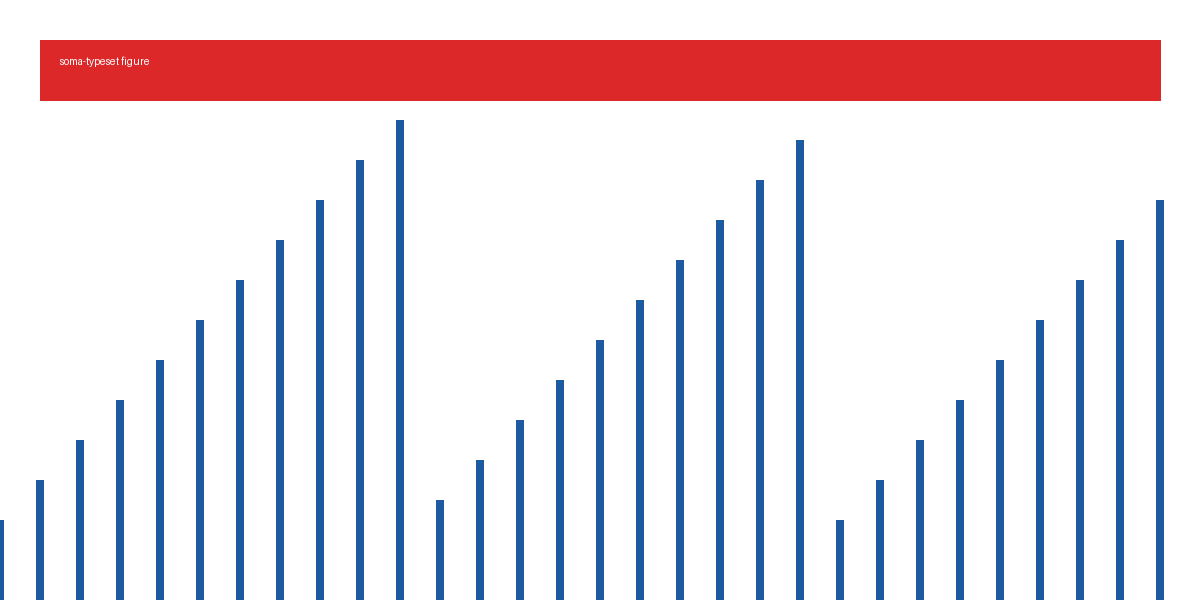
\includegraphics[width=0.9\linewidth]{fig/pipeline.png}
\caption{一张 PNG 位图：柱状图用来检查像素是否被正确解码}
\end{figure}

\begin{figure}
\centering
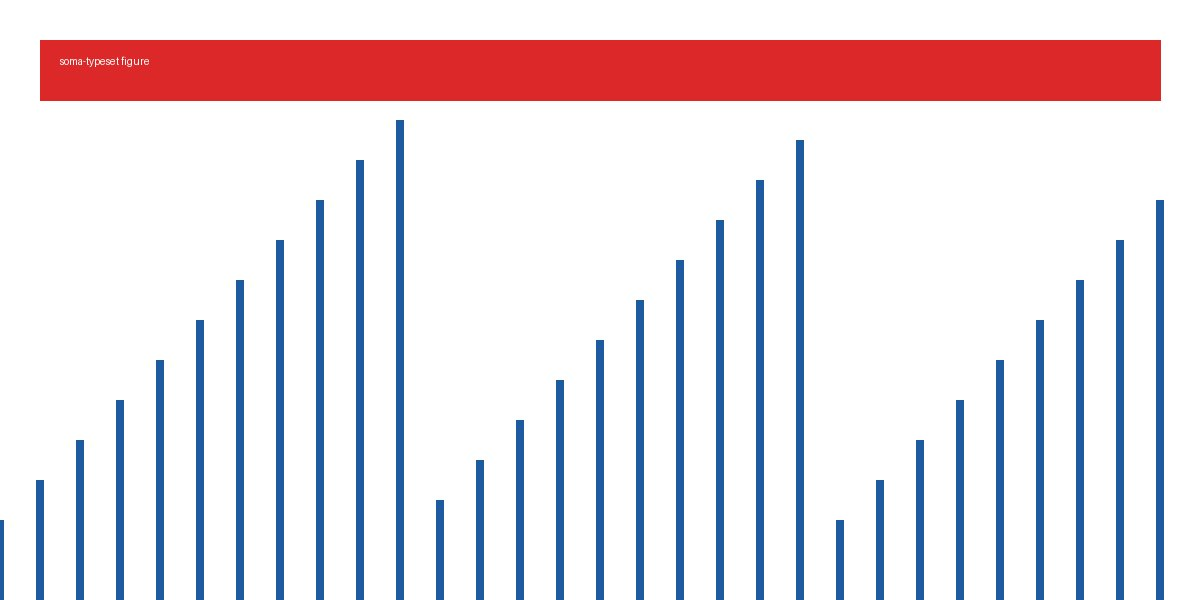
\includegraphics[width=0.8\linewidth]{fig/photo.jpg}
\caption{一张 JPEG 位图：走 \texttt{/DCTDecode} 直通，不解码像素}
\end{figure}

图题在图下方，居中小一号；图与图之间留出一行的空隙，避免两张图在视觉上粘成一张。

\section{表格与公式}

表格是这个引擎里最“结构化”的部分：列宽先按列数平分版心，再做行内断行，最后取行高的最大值。跨列单元格在计算占位时按列宽之和处理，跨行单元格则让它所在的行带变高，后续行依次顺延。

\begin{table}
\caption{字族、字重与用途}
\begin{tabular}{lll}
\hline
字族 & 字重 & 用途 \\
\hline
宋体 & 常规 & 正文 \\
宋体 & 粗体 & 正文强调 \\
\multicolumn{2}{l}{黑体（任意字重）} & 标题 \\
\hline
\end{tabular}
\end{table}

独立公式单独成块，居中，上下各留一点空隙：

\[
E = mc^2
\]

求和号在显示样式下把上下限排在符号的上下，而不是右侧：

\[
\sum_{i=1}^{n} a_i x^i
\]

分式与根号也已经有自己的几何：分数线是真实的矩形，根号的横线压在被开方数上方，两者嵌套时各层基线互不干扰：

\[
\frac{\sqrt{\pi}}{2}
\]

这些几何都由公式盒子自己算好，页面只负责把它放在基线上。

\section{脚注与索引}

脚注\footnote{脚注的高度会反过来影响它所在页面的可用空间，因此必须和正文一起求解，而不能先排正文再补脚注。}是长文档里最容易出错的部分：它改变页面剩余空间，而页面剩余空间又决定正文在哪里断开。这里的实现把脚注当作页面的固定开销，迭代若干轮直到页面高度稳定。

索引\index{索引}词条在正文里标记，在文末汇总。词条按 Unicode 码位排序，同一词条出现在多页时页码合并成列表。这份样张在“宋体”“索引”“表格”三处做了标记，可以看到文末的索引页。

\begin{verbatim}
soma render --input song.tex \
  --template song.yaml \
  --metrics song.smt \
  --format pdf --out song.pdf
\end{verbatim}

上面这段是等宽块，用来说明命令行的用法。等宽块不做断行，也不做首行缩进；如果某一行超出栏宽，宁可让它溢出，也不在命令中间插入换行——因为复制出去的必须是能跑的命令。

\section{小结}

把这份样张和之前的黑体版本对比，能看到三件事：宋体的字面更松，同样版心容量下每行字数略少；宋体的标点侧空更大，行末的空白更明显；宋体在相同字号下的视觉重量更轻，正文的“灰度”更均匀。这三件事都不是调参能解决的，它们是字体本身的属性，而排版引擎应该如实反映，而不是抹平。

真正需要引擎保证的是：换字体只换一张表，断行、分页、标点、索引、书签、结构标记全部照旧。这份文档就是这条承诺的验收样例。

\end{document}
